\documentclass[12pt,a4paper]{article}

% Paquetes básicos
\usepackage[utf8]{inputenc}
\usepackage{amsmath, amssymb, amsthm}
\usepackage{geometry}
\usepackage{hyperref}
\usepackage{enumitem}
\usepackage{etoolbox}
\usepackage{graphicx}
\usepackage{setspace}
\usepackage{tcolorbox}
\tcbuselibrary{skins, breakable}
\usepackage{titlesec}
\usepackage{tikz} % core TikZ
\usetikzlibrary{matrix}
\usepackage[x11names]{xcolor}

% Margins
%\geometry{left=3cm,right=3cm,top=2.5cm,bottom=2.5cm}

% Custom operators
\newcommand{\card}{\operatorname{card}}

% Implication box setup
\tcbset{Implication-number/.style={
  enhanced,
  boxsep=2pt,
  colback=white,
  frame hidden,
  sharp corners,
  left=2pt, right=2pt, top=1pt, bottom=1pt,
  underlay={
    \draw[line width=0.5pt] (frame.south west) -- ([xshift=-133mm]frame.south east); % línea horizontal
    \draw[line width=0.5pt] ([xshift=-133mm]frame.north east) -- ([xshift=-133mm]frame.south east); % línea vertical
  }
}}

\tcbset{Subset-contingency/.style={
  enhanced,
  boxsep=2pt,
  colback=white,
  frame hidden,
  sharp corners,
  left=2pt, right=2pt, top=1pt, bottom=1pt,
  underlay={
    \draw[line width=0.5pt] (frame.south west) -- ([xshift=-140mm]frame.south east); % línea horizontal
    \draw[line width=0.5pt] ([xshift=-140mm]frame.north east) -- ([xshift=-140mm]frame.south east); % línea vertical
  }
}}

% Useful commands
\renewcommand{\contentsname}{Contenidos}

\newcommand{\R}{\mathbb{R}}
\newcommand{\N}{\mathbb{N}}
\newcommand{\Z}{\mathbb{Z}}
\newcommand{\Q}{\mathbb{Q}}
\newcommand{\C}{\mathbb{C}}

\newcommand{\smallcup}{\mathop{\cup}\limits}
\newcommand{\smallcap}{\mathop{\cap}\limits}
\newcommand{\mlim}[1]{\displaystyle{\lim_{#1}}}


% ----- Custom counters and counter commands -----
% Custom counter hierarchy
\newcounter{unit}[section]
\newcounter{chapter}[unit]
\makeatletter
\@addtoreset{subsubsection}{chapter}
\makeatother

\renewcommand{\theunit}{\arabic{unit}}
\renewcommand{\thechapter}{\arabic{chapter}}
\renewcommand{\thesubsubsection}{\theunit.\thechapter.\arabic{subsubsection}}

% Custom content hierarchy behavior
\newcommand{\chapter}[1]{
    \refstepcounter{chapter}
    \subsection*{\Large{\S \thechapter. #1}}
    \addcontentsline{toc}{subsection}{\thechapter. #1}
}
\newcommand{\unit}[1]{
    \refstepcounter{unit}
    \section*{\Huge{\Roman{unit} #1}}
    \addcontentsline{toc}{section}{\Roman{unit} #1}
}

\newcommand{\result}[1]{%
  \subsubsection{#1}%
  \label{result:\thesubsubsection}
}
  
\titleformat{\subsubsection}
    {\normalfont\large\bfseries} % mismo tamaño que \subsection
    {\thesubsubsection}{1em}{}
  
%---- Custom proof commands-----
\newcommand{\dem}{
    \noindent \underline{\textbf{Demostración:}}
}
\newcommand{\nota}{
    \noindent \underline{\textbf{Nota:}}
}
% ----------------------------------------

\title{Análisis Matemático III}
\author{Javier Ortín Rodenas}
\date{Curso 2025-2026}

\begin{document}

\maketitle
\newpage
\tableofcontents
\newpage

\section*{\Huge{Introducción de la asignatura}}
\hspace{3mm}
\onehalfspacing
La materia será la misma que en años anteriores, aunque habrá un cambio en la metodología de enseñanza: no habrá tutorías grupales. No obstante, sí habrá evaluación continua. Su funcionamiento se explicará posteriormente.

%TODO: placeholder for evaluación continua

\newpage

\section*{\Huge{Preliminares}}
\phantomsection \addcontentsline{toc}{section}{Preliminares}
En la sección de preliminares se tratarán los siguientes temas:
\begin{itemize}
    \item Cardinalidad de conjuntos
    \item Descomposición de abiertos de $\R^N$ en unión de cubos diádicos
    \item Series dobles
\end{itemize}

\vspace{2mm}

\chapter{Cardinalidad de conjuntos}

\vspace{2mm}

\result{Definición de cardinalidad, tipos de cardinalidad}
\hspace{3mm}
Intuitivamente, podemos definir la cardinalidad de un conjunto como el número de elementos que tiene. Además, es lógico plantear la distinción entre conjuntos finitos e infinitos. Veamos cómo formalizar esta idea.

\vspace{2mm}

Sea $A$ un conjunto no vacío, diremos que $A$ es un conjunto finito de cardinalidad $n \in \N = \{1,2,\ldots\}$ si existe una aplicación biyectiva $\varphi : \{1,2,\ldots,n\} \to A$.

\noindent Se considera que el conjunto vacío $\varnothing$ es finito con cardinal $0$.

\vspace{4mm}

Sea $A$ un conjunto cualquiera, diremos que es un conjunto infinito si existe cierta aplicación inyectiva $\varphi : \N \to A$. Dentro de esta clasificación, diremos que $A$ es infinito numerable si existe una aplicación $\varphi : \N \to A$ biyectiva. Si esto último no fuese posible, diremos que $A$ es infinito no numerable.

\vspace{4mm}

Aunque no entra dentro de los objetivos de esta asignatura, es interesante contemplar la siguiente observación: Si un conjunto no es un conjunto finito, podemos afirmar simplemente que es un conjunto "no finito". Si además incluimos el axioma de elección, sí podremos afirmar que tal conjunto es infinito. Dentro de los conjuntos infinitos, todos son o bien numerables o bien no numerables, sin intersección entre ambas categorías.

\vspace{4mm}

\result{Ejemplos de conjuntos numerables}

$\bullet$ $\N$: trivial, basta considerar la aplicación identidad. \\

\noindent
$\bullet$ $\Z$: basta considerar la siguiente aplicación biyectiva:

%Function definition and mapping side by side
\begin{minipage}{0.5\textwidth}
    \begin{align*}
    \varphi(n) =
    \begin{cases}
    \frac{n}{2}, & \text{si } n \text{ es par} \\
    -\frac{n-1}{2}, & \text{si } n \text{ es impar}
    \end{cases}
    \end{align*}
\end{minipage}%
\begin{minipage}{0.5\textwidth}
    \begin{align*}
    \begin{array}{cccccc}
    1 & 2 & 3 & 4 & 5 & \cdots \\
    \downarrow\!\varphi & \downarrow\!\varphi & \downarrow\!\varphi & \downarrow\!\varphi & \downarrow\!\varphi & \\
    0 & 1 & -1 & 2 & -2 & \cdots
    \end{array}
    \end{align*}
\end{minipage}

\vspace{7mm}

\noindent $\bullet$ $\Q := \left\{\frac{z}{n} : z \in \Z, n \in \N \right\}$. Denotaremos por $\hat{Q}$ al conjunto $\left\{\frac{z}{n} : z,n \in \N\right\}$. Como hemos visto en el apartado anterior, al ser $\Z$ numerable, $\hat{Q}$ y $\Q$ han de tener necesariamente la misma cardinalidad. Por tanto, basta con demostrar que $\hat{Q}$ es numerable, lo que haremos a continuación por medio de una doble desigualdad.

\vspace{2mm}

\phantomsection \label{racionales-numerables}
Representaremos los elementos de $\hat{Q}$ en una tabla infinita que recorreremos diagonalmente:
\begin{center}
    \scalebox{0.9}{ %downscale the tikzpicture
    \begin{tikzpicture}[baseline=(current bounding box.center)]
    % Draw the table with extra space for lines
    \matrix (m) [matrix of math nodes, nodes in empty cells, row sep=8mm, column sep=10mm, ampersand replacement=\&, cells={nodes={minimum width=1.5em, minimum height=2.5ex, anchor=center, text height=1.5ex, text depth=.25ex}} ]{
    {} \& 1 \& 2 \& 3 \& 4 \& \ldots \\
    1 \& \frac{1}{1} \& \frac{2}{1} \& \frac{3}{1} \& \frac{4}{1} \& \ldots \\
    2 \& \frac{1}{2} \& \frac{2}{2} \& \frac{3}{2} \& \frac{4}{2} \& \ldots \\
    3 \& \frac{1}{3} \& \frac{2}{3} \& \frac{3}{3} \& \frac{4}{3} \& \ldots \\
    4 \& \frac{1}{4} \& \frac{2}{4} \& \frac{3}{4} \& \frac{4}{4} \& \ldots \\
    \vdots \& \vdots \& \vdots \& \vdots \& \vdots \& \ddots \\
    };
    % Draw horizontal line below header row
    \draw[thick] ([xshift=-4mm, yshift=-2mm]m-1-1.south west) -- ([xshift=7mm, yshift = -2mm]m-1-6.south east);
    % Draw vertical line after header column
    \draw[thick] ([xshift =4mm ,yshift=5mm]m-1-1.north east) -- ([xshift=4mm, yshift=-5mm]m-6-1.south east);

    % Draw diagonal arrows
    \draw[->, thick, red] ([xshift=2mm, yshift=2mm]m-2-2.north east) -- (m-2-2) -- ([xshift=-2mm, yshift=-2mm]m-2-2.south west); % 1st diagonal (1/1
    \draw[->, thick, red] ([xshift=2mm, yshift=2mm]m-2-3.north east) --(m-2-3) -- (m-3-2) -- ([xshift=-2mm, yshift=-2mm]m-3-2.south west); % 2nd diagonal (2/1 to 1/2)
    \draw[->, thick, red] ([xshift=2mm, yshift=2mm]m-2-4.north east) --(m-2-4) -- (m-3-3) -- (m-4-2) -- ([xshift=-2mm, yshift=-2mm]m-4-2.south west) ; % 3rd diagonal (3/1 to 1/3)
    \draw[->, thick, red] ([xshift=2mm, yshift=2mm]m-2-5.north east) -- (m-2-5) -- (m-3-4) -- (m-4-3) -- (m-5-2)-- ([xshift=-2mm, yshift=-2mm]m-5-2.south west); % 4th diagonal (4/1 to 1/4)

    % Add more diagonals if needed
    \end{tikzpicture}
    }
\end{center}
Por tanto, obtenemos como resultado la siguiente aplicación
$\varphi : \N \to \hat{Q}$ con
$$\varphi(1) = \frac{1}{1}, \hspace{4mm} \varphi(2) = \frac{2}{1}, \hspace{4mm}
\varphi(3) = \frac{1}{2},  \hspace{4mm} \varphi(4) = \frac{3}{1}, \hspace{4mm}
\varphi(5) = \frac{2}{2},  \hspace{4mm} \varphi(6) = \frac{1}{3}\ldots$$

Aunque esta aplicación no es inyectiva (por ejemplo $\varphi(1) = \varphi(5)$), sí es suprayectiva.
Por tanto, $\card\N \leq \card\hat{Q}$. Además, como $\N \subseteq \hat{Q}$, es evidente que $\card\N \geq \card\hat{Q}$.
En consecuencia, $\card\N = \card\hat{Q}$; es decir, $\hat{Q}$ es numerable y por tanto también lo es $\Q$.

\vspace{2mm}
\result{Ejemplos de conjuntos no numerables}
\hspace{3mm}
Vemos que $\R$ es no numerable por reducción al absurdo. Supongamos que existe una aplicación biyectiva $\varphi : \N \to \R$.
Así, ha de cumplirse $\varphi(\N) = \R$. Definiremos una sucesión de intervalos encajados como sigue:
\begin{itemize}
    \item Tomamos $a_1, b_1$ cualesquiera tales que $a_1 < b_1$ y $\varphi(1) \notin [a_1, b_1]$
    \item Para $n > 1$, tomamos $a_n, b_n$ tales que  $a_n < b_n$, $[a_n, b_n] \subset (a_{n-1}, b_{n-1})$ y $\varphi(n) \notin [a_n, b_n]$
\end{itemize}
De este modo, obtenemos una sucesión de intervalos cerrados encajados tales que $\varphi(n) \notin [a_n, b_n] \hspace{1mm} \forall n \in \N$.
Denotando $I_i = [a_i, b_i]$, se cumple:
\begin{enumerate}
    \item $I_1$ es compacto por el teorema de Heine-Borel
    \item $\{I_n : n \in \N\}$ verifica la propiedad de la intersección finita
\end{enumerate}
Al ser una sucesión de intervalos cerrados encajados, juntando las dos nociones anteriores, podemos
afirmar que se satisface la propiedad de la intersección infinita. Por tanto, se tiene:
\\[-2ex]
$$\exists \hspace{2mm} x_0 \in \bigcap_{n=1}^{\infty} I_n
\Rightarrow x_0 \in \R \backslash \varphi(\N)
\Rightarrow \varphi(\N) \neq \R
\Rightarrow \varphi \text{ no es biyectiva}$$
Se contradice la hipótesis de partida. Por todo lo anterior, concluimos que $\R$ es no numerable.

\vspace{6mm}
La aplicación $\tan : (-\frac{\pi}{2}, \frac{\pi}{2}) \longrightarrow \R$ es biyectiva, luego el intervalo
$(-\frac{\pi}{2}, \frac{\pi}{2})$ es no numerable. Por otro lado, podemos establecer una biyección entre
este intervalo y cualquier otro intervalo abierto. Así, cualquier intervalo es no numerable.

\result{Procesos que dan lugar a conjuntos numerables}
\hspace{3mm}
Sea $A$ un conjunto finito, sea $B$ un conjunto infinito numerable. Entonces,
$A \cup B$ y $A \times B$ son conjuntos infinitos numerables (o vacíos).

\vspace{4mm}
\dem Distinguiremos dos casos:

\vspace{2mm}
Si $A = \varnothing$, entonces $A \cup B = B$ que es infinito numerable por hipótesis.
Además, $A \times B = \varnothing$ que es finito por definición.

\vspace{4mm}
Si $A \neq \varnothing$, como $A$ es finito podemos afirmar que $A\backslash B = \{a_1, a_2, \ldots, a_{n_1}\}$
para cierto $n_1 \in \N \cup \{0\}$. Por ser $B$ infinito numerable, existe una aplicación biyectiva $\varphi : \N \to B$.
Para ver que $A \cup B$ es infinito numerable, basta considerar la siguiente biyección:
\begin{align*}
    \hat{\varphi} (n) = \begin{cases}
    a_n, & \text{si } n \leq n \leq n_1 \\
    \varphi(n - n_1), & \text{si } n > n_1
    \end{cases}
\end{align*}
Esta biyección $\hat{\varphi}$ enumera primero todos los elementos de $A \backslash B$ (de haberlos)
para luego enumerar todos los elementos de $B$ en el orden original de $\varphi$.

\vspace{4mm}
Al ser $A$ finito, podemos escribir $A = \{a_1, a_2, \ldots, a_{n_2}\}$ para cierto $n_2 \in \N$.
Para ver que $A \times B$ es infinito numerable, podemos enumerar sus elementos de la siguiente forma:
\begin{center}
\begin{tabular}{c|cccc}
    & 1 & 2 & \ldots & $n_2$ \\
    \hline
    1 & $(a_1, \varphi(1))$ & $(a_2, \varphi(1))$ & $\ldots$ & $(a_{n_2}, \varphi(1))$ \\
    2 & $(a_1, \varphi(2))$ & $(a_2, \varphi(2))$ & $\ldots$ & $(a_{n_2}, \varphi(2))$ \\
    3 & $(a_1, \varphi(3))$ & $(a_2, \varphi(3))$ & $\ldots$ & $(a_{n_2}, \varphi(3))$ \\
    $\vdots$ & $\vdots$ & $\vdots$ & & $\vdots$ \\
\end{tabular}
\end{center}
\vspace{2mm}
Basta enumerar los elementos de $A \times B$ recorriendo la tabla de izquierda a derecha y de arriba a abajo,
pues cada fila tiene $n_2$ elementos y hay tantas filas como naturales.

\result{Más procesos que dan lugar a conjuntos numerables}
\hspace{3mm}
Sean $A, B$ conjuntos infinitos numerables con $A \cap B = \varnothing$.
Entonces, $A \cup B$ y $A \times B$ son conjuntos infinitos numerables.

\vspace{4mm}
\dem Al ser $A$ y $B$ infinitos numerables por hipótesis, podemos afirmar que existen ciertas
aplicaciones biyectivas \hspace{1mm} $\varphi_A : \N \to A$ \hspace{1mm} y \hspace{1mm} $\varphi_B : \N \to B$.

\vspace{2mm} \noindent
Para ver que $A \cup B$ es infinito numerable, basta considerar la siguiente biyección:
\\[-4ex]
\begin{align*}
    \varphi_{A \cup B} (n) =
    \begin{cases}
        \varphi_A\left(\frac{n+1}{2}\right), & \text{si } n \text{ es impar} \\
        \varphi_B\left(\frac{n}{2}\right), & \text{si } n \text{ es par}
    \end{cases}
\end{align*}
Así, se enumeran alternativamente los elementos de $A$ y $B$. Al ser $A \cap B = \varnothing$,
es seguro que esta aplicación es biyectiva.

\vspace{4mm}
Finalmente, para ver que $A \times B$ es infinito numerable, podemos representar sus elementos de forma matricial
utilizando un razonamiento diagonal análogo al empleado para ver que \hyperref[racionales-numerables]{$\Q$ es numerable}.

\vspace{6mm}
\nota Aunque en esta demostración hemos supuesto que $A \cap B = \varnothing$, el resultado puede aplicarse también para conjuntos
de intersección no vacía. Nótese que como $A$ y $B$ son infinito numerables, entonces $A \cap B, \hspace{1mm} A \backslash B$ y $B \backslash A$
han de ser necesariamente conjuntos finitos o infinitos numerables. Finalmente, basta ver que
$A \cup B =\big((A\backslash B) \cup (B \backslash A) \big) \cup (A \cap B)$, unión de conjuntos disjuntos.
Como para el caso del producto cartesiano no se ha usado la hipótesis
de que $A \cap B = \varnothing$, el resultado es válido en cualquier caso.
%TODO: union numerable de conjuntos numerables

\vspace{6mm}
\result{Unión numerable de conjuntos numerables}
\hspace{3mm}
Sea $\{A_n : n \in \N\}$ una colección de conjuntos numerables, entonces su unión
es también un conjunto numerable.

\vspace{4mm}
\dem Utilizaremos también un argumento diagonal.
\newpage

De manera similar a la demostración anterior, expresaremos la unión $\bigcup_{n \in \N} A_n$ a partir de conjuntos
auxiliares disjuntos para simplificar el trato de los elementos duplicados:
\vspace{-2mm}
\begin{itemize}
    \item Para $n = 1$, definimos $B_1 := A_1$
    \item Para $n > 1$, definimos $B_n := A_n \backslash \left(\bigcup_{k=1}^{n-1}A_k\right) = A_n \backslash B_{n-1}$
\end{itemize}
De este modo, los $B_i$ son disjuntos entre sí. Además, todos los $A_i$ son numerables por hipótesis, cada $B_i$ 
ha de ser finito o numerable. Según el carácter de cada uno de ellos, introducimos la siguiente notación:
\begin{align*}
    \text{Caso finito: } B_i = \big\{b^i_1, b^i_2, \ldots, b^i_{n_i} \big\} &&
    \text{Caso numerable: } B_j = \bigcup_{n \in \N}b^j_n
\end{align*}
Con esta notación, expresaremos los elementos de cada $B_i$ tabularmente:
\begin{center}
    \scalebox{0.9}{ %downscale the tikzpicture
    \begin{tikzpicture}[baseline=(current bounding box.center)]
    % Draw the table with extra space for lines
    \matrix (m) [matrix of math nodes, nodes in empty cells, row sep=8mm, column sep=10mm, ampersand replacement=\&, cells={nodes={minimum width=1.5em, minimum height=2.5ex, anchor=center, text height=1.5ex, text depth=.25ex}} ]{
    {} \& B_1 \& B_2 \& B_3 \& B_4 \& \ldots \\
    1 \& b^1_1 \& b^2_1 \& b^3_1 \& b^4_1 \& \ldots \\
    2 \& b^1_2 \&       \& b^3_2 \& b^4_2 \& \ldots \\
    3 \& b^1_3 \&       \& b^3_3 \& b^4_3 \& \ldots \\
    4 \& b^1_4 \&       \& b^3_4 \& b^4_4 \& \ldots \\
    \vdots \& \vdots \&  \& \vdots \& \vdots \& \ddots \\
    };
    % Draw horizontal line below header row
    \draw[thick] ([xshift=-4mm, yshift=-2mm]m-1-1.south west) -- ([xshift=7mm, yshift = -2mm]m-1-6.south east);
    % Draw vertical line after header column
    \draw[thick] ([xshift =4mm ,yshift=5mm]m-1-1.north east) -- ([xshift=4mm, yshift=-5mm]m-6-1.south east);

    % Draw diagonal arrows
    \draw[->, thick, red] ([xshift=2mm, yshift=2mm]m-2-2.north east) -- (m-2-2) -- ([xshift=-2mm, yshift=-2mm]m-2-2.south west); % 1st diagonal (1/1
    \draw[->, thick, red] ([xshift=2mm, yshift=2mm]m-2-3.north east) --(m-2-3) -- (m-3-2) -- ([xshift=-2mm, yshift=-2mm]m-3-2.south west); % 2nd diagonal (2/1 to 1/2)
    \draw[->, thick, red] ([xshift=2mm, yshift=2mm]m-2-4.north east) --(m-2-4) -- (m-4-2) -- ([xshift=-2mm, yshift=-2mm]m-4-2.south west) ; % 3rd diagonal (3/1 to 1/3)
    \draw[->, thick, red] ([xshift=2mm, yshift=2mm]m-2-5.north east) -- (m-2-5) -- (m-3-4) -- (m-5-2)-- ([xshift=-2mm, yshift=-2mm]m-5-2.south west); % 4th diagonal (4/1 to 1/4)

    % Add more diagonals if needed
    \end{tikzpicture}
    }
\end{center}
Recorremos diagonalmente la matriz, saltando las celdas vacías en caso de haberlas (ocurriría en caso de que algún $B_i$ fuese finito).
Por ejemplo, el $B_2$ de la figura tiene tan solo un único elemento. Como hemos tomado $B_1 = A_1$, hay infinitos elementos al ser $A_1$
infinito numerable por hipótesis (no pueden ser finitos todos los $B_i$).

\vspace{6mm}
\result{Definición de conjunto de partes}
\hspace{3mm}
Sea $A$ un conjunto cualquiera, se denomina "conjunto de partes de $A$" y se denota como $\mathcal{P}(A)$
al conjunto cuyos elementos son todos los subconjuntos de $A$. En particular, siempre se cumple
que $\varnothing, A \in \mathcal{P}(A)$.

\vspace{2mm} \noindent
Por ejemplo, para $A = \{1,2\}$, se tiene que $\mathcal{P}(A) = \big\{\varnothing, \{1\}, \{2\}, \{1,2\} \big\}$.

\vspace{6mm}
\result{Cardinal de partes de un conjunto finito}
\hspace{3mm}
Sea $A$ un conjunto finito, entonces $\card \mathcal{P}(A) = 2^{\text{} \card A} \in \N$.

\vspace{4mm}
\dem Distinguiremos dos casos:

\vspace{2mm} \noindent
Para $A = \varnothing$, se tiene que $\mathcal{P}(A) = \{\varnothing\}$, luego $\card \mathcal{P}(A) = 1 = 2^0 = 2^{\text{} \card A}$.

\vspace{4mm}
Si $A \neq \varnothing$, sea $n := \card A \in \N$, podemos identificar cada subconjunto de $A$ según la presencia o ausencia de cada uno de sus $n$ elementos.
Definimos el conjunto de las tuplas de ceros y unos de longitud $n$ como sigue:
\vspace{-1ex}
$$C := \big\{(\varepsilon_1 , \ldots, \varepsilon_n) : \varepsilon_i \in \{0,1\} \hspace{2mm} \forall i \in \{1,\ldots,n\}\big\}$$
Así, denotando $A = \{a_1, \ldots, a_n\}$, cada tupla de $C$ puede asociarse biunívocamente a un subconjunto de $A$ al indicar cada
$\varepsilon_i$ si el elemento $a_i$ pertenece o no al subconjunto. Por tanto, la siguiente aplicación $\varphi$ es biyectiva:
\[
\begin{aligned}
    &\varphi : \mathcal{P}(A) \longrightarrow C \\
    &\hspace{6mm} B \longmapsto \prod_{i=1}^{n} f_i(B)
\end{aligned}
\hspace{10mm}
\text{donde}
\hspace{10mm}
\begin{aligned}
    &f_i : \mathcal{P}(A) \longrightarrow \{0,1\} \\
    &\hspace{6mm} B \longmapsto
    \begin{cases}
        1, & \text{si } a_i \in B \\
        0, & \text{si } a_i \notin B
    \end{cases}
\end{aligned}
\]

\vspace{6mm}
\result{El conjunto de partes incrementa la cardinalidad}
\hspace{3mm}
Sea $A$ un conjunto cualquiera. Entonces, $\card A < \card \mathcal{P}(A)$.

\vspace{4mm}
\dem Para todo conjunto $A$ se cumple que $\card A \leq \card \mathcal{P}(A)$,
pues $a \in A \Rightarrow \{a\} \in \mathcal{P}(A)$. Veamos ahora que no puede darse
la igualdad por reducción al absurdo.

\vspace{2mm}
Supongamos que existe un conjunto $A$ tal que $\card \mathcal{P}(A) = \card A$.
En tal caso, ha de existir una aplicación biyectiva $\varphi : A \to \mathcal{P}(A)$.
A partir de ella definimos el siguiente conjunto auxiliar: $B := \{a \in A : a \notin \varphi(a)\}$.
Por construcción, $B$ es un subconjunto de $A$, luego $B \in \mathcal{P}(A)$. Al ser $\varphi$ biyectiva,
existe cierto $z \in A$ tal que $\varphi(z) = B$.

\noindent
Pueden darse dos casos:
\begin{enumerate}[label=\arabic*.)]
    \item $z \in B = \varphi(z) \Rightarrow z \notin \varphi(z) = B$, contradicción.
    \item $z \notin B = \varphi(z) \Rightarrow z \in B = \varphi(z)$, contradicción
\end{enumerate}
En cualquiera de ellos se llega a una contradicción. Por todo lo anterior, concluimos que $\card A < \card \mathcal{P}(A)$.

\vspace{6mm}
\result{Cardinalidad de \texorpdfstring{$\mathcal{P}(\N)$}{P(N)}}
\hspace{3mm} De manera similar a \hyperref[racionales-numerables]{como hicimos para ver el cardinal de un conjunto finito}, podemos identificar cada
subconjunto de $\N$ en base a la presencia o ausencia de cada número natural en tal conjunto. Así, sabemos que existe una biyección entre los subconjuntos
de $\N$ y las sucesiones formadas por ceros y unos:
$$\varphi : \mathcal{P}(\N) \longrightarrow \big\{0,1\big\}^\N = \Big\{(\varepsilon_n)_{n \in \N} : \varepsilon_i \in \{0,1\} \hspace{2mm}  \forall i \in \N\Big\}$$
Además, podemos asociar cada sucesión de ceros y unos a la expresión en base 2 de un número real del intervalo $[0,1]$. Aplicando lo visto en los
resultados \hyperref[result:0.1.3]{0.1.3} y \hyperref[result:0.1.4]{0.1.4}, tal intervalo tiene la misma cardinalidad que $\R$; es decir, $2^{\aleph_0}$.

\vspace{6mm}
\result{Jerarquía de cardinalidades}
\hspace{3mm}    
En vista de los resultados anteriores, podemos establecer una jerarquía de cardinalidades. En primer lugar, está el conjunto vacío (de cardinal cero).
A continuación, los conjuntos finitos de cardinal natural. Pasando ahora a los conjuntos infinitos, la menor cardinalidad posible es la de los conjuntos
infinitos numerables, denotada por $\aleph_0$. Como consecuencia del resultado \hyperref[result:0.1.9]{0.1.9}, sabemos que podemos encontrar conjuntos
de cardinalidad cada vez mayor al considerar el conjunto de partes de la iteración anterior.

\vspace{2mm}
Cabe preguntarse si existe algún tipo de cardinalidad intermedia entre los infinitos de esta escala. Esta cuestión es la conocida como
Hipótesis del Continuo (CH), y se sabe que no puede ser probada ni refutada a partir de los axiomas habituales de la teoría de conjuntos (ZFC). 
Por tanto, debe considerarse como un axioma adicional independiente de ZFC: el axioma del continuo.

\vspace{10mm}
\chapter{Descomposición de subconjuntos abiertos de \texorpdfstring{$\R^N$}{R\^N} en cubos diádicos}
\vspace{4mm}
\result{Definición de intervalo diádico}
\hspace{3mm}
Se llama "intervalo diádico de orden $n$" con $n \in \N$ a cualquier intervalo
real de la forma $\Big[\frac{j-1}{2^n}, \frac{j}{2^n}\Big)$ con $j \in \Z$.

\vspace{4mm}
\result{Propiedades de los intervalos diádicos}
\hspace{3mm}
Fijado $n \in \N$ cualquiera, se tiene que la colección de todos los intervalos diádicos de orden $n$
es numerable (pues hay uno por cada $j \in \Z$) y recubre $\R$:
$$\bigcup_{j \in \Z} \Big[\frac{j-1}{2^n}, \hspace{1mm}  \frac{j}{2^n}\Big) = \R$$
Además, dos intervalos diádicos cualesquiera son disjuntos o bien coinciden:
$$i \neq j \Rightarrow \Big[\frac{i-1}{2^n}, \frac{i}{2^n} \Big) 
\bigcap \Big[\frac{j-1}{2^n}, \frac{j}{2^n}\Big) = \varnothing $$

Las dos propiedades anteriores pueden visualizarse en la siguiente figura:
\vspace{2mm}
\begin{center}
    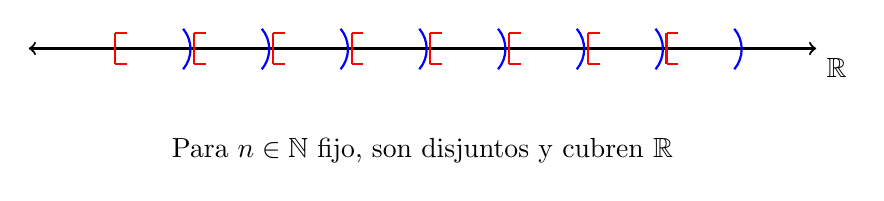
\begin{tikzpicture}
        % Draw the number line
        \draw[thick,<->] (-5,0) -- (5,0) node[anchor=north west] {$\R$};

        % Draw the dyadic intervals of order n=3
        \foreach \j in {-4,...,3} {
            % Draw interval [
            \draw[-, red, thick] (\j+0.1, -0.2) -- (\j+0.1, 0.2);
            \draw[-, red, thick] (\j+0.1, -0.2) -- (\j+0.25, -0.2);
            \draw[-, red, thick] (\j+0.1, 0.2) -- (\j+0.25, 0.2);

            %Draw interval )
            \draw[-, blue, thick] (\j+0.96, 0.25) arc [start angle =40, end angle = -40, radius=0.4];
        }

        % Label the intervals
        \node at (0,-1.3) {Para $n \in \N$ fijo, son disjuntos y cubren $\R$};
    \end{tikzpicture}
\end{center}

\vspace{2mm}
Si $I$ es un intervalo diádico de orden $n$ y $J$ es un intervalo diádico
de orden $m \in \N$ con $m \leq n$: entonces se cumple:
\begin{align*}
    \bullet \hspace{2mm} \text{O bien } I \subsetneq J &&
    \bullet \hspace{2mm} \text{O bien } I \cap J = \varnothing
\end{align*}
La siguiente figura ilustra este hecho:
\vspace{2mm}
\begin{center}
    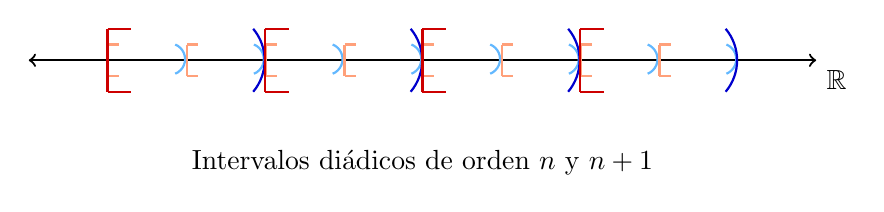
\begin{tikzpicture}
        % Draw the number line
        \draw[thick,<->] (-5,0) -- (5,0) node[anchor=north west] {$\R$};

        % Draw the dyadic intervals of order n=3
        \foreach \j in {-4,...,3} {
            % Draw interval [
            \draw[-, LightSalmon1, thick] (\j+0.01, -0.2) -- (\j+0.01, 0.2);
            \draw[-, LightSalmon1, thick] (\j+0.01, -0.2) -- (\j+0.15, -0.2);
            \draw[-, LightSalmon1, thick] (\j+0.01, 0.2) -- (\j+0.15, 0.2);

            %Draw interval )
            \draw[-, SteelBlue1, thick] (\j+0.86, 0.2) arc [start angle =68, end angle = -68, radius=0.2];
        }

        \foreach \j in {-4, -2, 0, 2} {
            % Draw interval [
            \draw[-, Red3, thick] (\j, -0.4) -- (\j, 0.4);
            \draw[-, Red3, thick] (\j, -0.4) -- (\j+0.3, -0.4);
            \draw[-, Red3, thick] (\j, 0.4) -- (\j+0.3, 0.4);

            %Draw interval )
            \draw[-, Blue3, thick] (\j+1.85, 0.4) arc [start angle =40, end angle = -40, radius=0.6222];
        }
        

        % Label the intervals
        \node at (0,-1.3) {Intervalos diádicos de orden $n$ y $n+1$};
    \end{tikzpicture}
\end{center}

\vspace{6mm}
\result{Definición de cubo diádico}
\hspace{3mm}
Llamamos "cubo diádico de $\R^N$ de orden $n$" con $n, N \in \N$ a cualquier conjunto de
la forma $I_1, \times I_2 \times \ldots \times I_N$ donde cada $I_i$ es un intervalo diádico de orden $n$.

\vspace{2mm} \noindent
Denotaremos por $\mathcal{F}_n$ al conjunto de todos los cubos diádicos de orden $n$ en $\R^N$.

\vspace{4mm}
\result{Propiedades de los cubos diádicos}
\hspace{3mm} Los cubos diádicos de orden $n$ son numerables y recubren $R^N$ (consecuencia de la definición y de los resultados anteriores).
Además, son disjuntos o coinciden; es decir:
\begin{align*}
    \left.
    \begin{array}{l}
        C \in \mathcal{F}_n \\
        D \in \mathcal{F}_n \\
        C \neq D
    \end{array}
    \right\}
    \Rightarrow C \cap D = \varnothing
\end{align*}
Como $C,D \in \mathcal{F}_m$, han de ser de la siguiente forma:
\vspace{-2mm}
\begin{align*}
    C = I_1 \times \ldots \times I_N &&
    D = J_1 \times \ldots \times J_N
\end{align*} \\[-5ex]
donde los $I_i$ y los $J_j$ son intervalos diádicos de orden $n$.
Por hipótesis, $C \neq D$ luego ha de existir cierto $k \in \{1, \ldots, n\}$
tal que $I_k \neq J_k$. Por las \hyperref[result:0.2.2]{propiedades de los intervalos diádicos},
sabemos que esto implica que $I_k \cap J_k = \varnothing$. Esto a su vez implica que $C \cap D = \varnothing $.

\vspace{4mm}
De manera similar, si $C \in \mathcal{F}_n, D \in \mathcal{F}_m$ con $m \leq n$. Entonces o bien
$C \subsetneq D$ o bien $C \cap D = \varnothing$. Por definición de $\mathcal{F}_n$ y $\mathcal{F}_m$,
podemos afirmar que:
\begin{align*}
    C = I_1 \times \ldots \times I_N  &&
    D = J_1 \times \ldots \times J_N
\end{align*}
Donde los $I_i$ y los $J_j$ son intervalos diádicos de orden $n$ y $m$, respectivamente. Por las
\hyperref[result:0.2.2]{propiedades de los intervalos diádicos}, para cada $k \in \{1, \ldots, N\}$ se tiene
que o bien $I_k \subsetneq J_k$ o bien $I_k \cap J_k = \varnothing$. Si $\exists k_0 \in \{1, \ldots, N\}$ tal que
$I_{k_0} \cap J_{k_0} = \varnothing$, entonces $C \cap D = \varnothing$. En caso contrario, $C \subsetneq D$.

\vspace{8mm}
\result{Teorema de descomposición de abiertos en cubos diádicos}
\hspace{3mm}
Para todo subconjunto no vacío y abierto en $\left(\R^N, \tau_{R^N}(d)\right)$, $O$, existe una colección numerable
de cubos diádicos (posiblemente de órdenes distintos) de $\R^N$, $\left\{C_n : n \in \N\right\}$, tales que:
\begin{enumerate}[label=\arabic*.)]
    \item $O$ = $\displaystyle \bigcup_{n \in \N} C_n$
    \item $\overline{C_n} \subseteq O \hspace{2mm} \forall n \in \N$
    \item $i \neq j \Rightarrow C_i \cap C_j = \varnothing$
\end{enumerate}

\vspace{4mm}
\dem Definiremos varios conjuntos auxiliares.

\vspace{2mm}
Definimos $\mathcal{G}_n := \left\{C \in \mathcal{F}_n : \overline{C} \subseteq O\right\}$. Cada una de estas colecciones de conjuntos
es finita o numerable al serlo $\mathcal{F}_n$.

\vspace{2mm}
A partir de los $\mathcal{G}_n$ definiremos otra colección de conjuntos.
Para $n = 1$, tomamos $\mathcal{H}_1 := \mathcal{G}_1$.
Para $n >1$, definimos
$$\mathcal{H}_n := \left\{C \in \mathcal{G}_n : C \nsubseteq \displaystyle \bigcup_{k=1}^{n-1}\mathcal{H}_k \right\}
= \left\{C \in \mathcal{G}_n : C \cap \left[\hspace{1mm} \bigcup_{k=1}^{n-1} \hspace{1mm} \bigcup_{D \in \mathcal{H}_k} D_k\right] = \varnothing \right\}$$
La última igualdad se deduce de las \hyperref[result:0.2.4]{propiedades de los cubos diádicos}.
Por construcción, los $\mathcal{H}_n$ son numerables y disjuntos entre sí. Además, por construcción, la clausura de sus cubos
está contenida en $O$. Queda probar el punto (1).

\vspace{2mm}
Intuitivamente, $\mathcal{G}_n$ modela los cubos 
de un cierto orden que ``caben" en $O$. El paso a los $\mathcal{H}_n$ hace que solo se empiecen a usar cubos ``más pequeños" en las zonas donde no ``cabrían"
cubos de un orden inferior (``más grandes").
\\[5ex]
%G_1
\begin{minipage}{0.50\textwidth}
    \begin{center}
    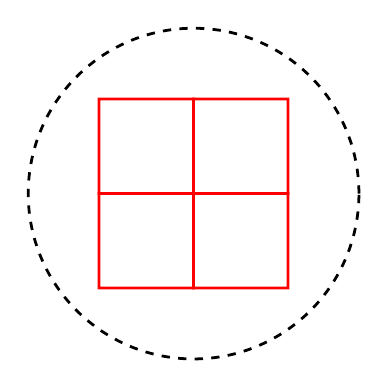
\begin{tikzpicture}[scale=0.6, blend group = normal]
        \draw[-, black, dashed] (0,0) circle (3.5);
        \foreach \i in {-2,0} {
            \foreach \j in {-2,0} {
                \draw[-, red] (\i,\j) rectangle (\i+2, \j+2);
            }
        }
    \end{tikzpicture}
    \\
    $\mathcal{G}_1$
    \end{center}
\end{minipage}
%G_2
\begin{minipage}{0.50\textwidth}
    \begin{center}
        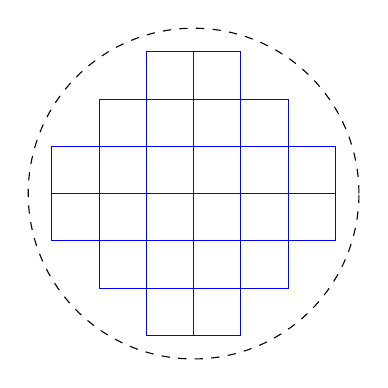
\begin{tikzpicture}[scale=0.6]
            \draw[-, black, dashed] (0,0) circle (3.5);
            \path[draw=blue]
            \foreach \i in {-2,...,1} {
                \foreach \j in {-2,...,1} {
                    (\i,\j) rectangle (\i+1,\j+1)
                }
            }
            \foreach \i in {-1,0} {
                \foreach \j in {-3,2} {
                    (\i,\j) rectangle (\i+1,\j+1)
                    (\j,\i) rectangle (\j+1,\i+1)
                }
            };
        \end{tikzpicture} \\
        $\mathcal{G}_2$
    \end{center}
\end{minipage}
\\[5ex]
%H_1
\begin{minipage}{0.33\textwidth}
    \begin{center}
    \begin{tikzpicture}[scale=0.6]
        \draw[-, black, dashed] (0,0) circle (3.5);
        \foreach \i in {-2,0} {
            \foreach \j in {-2,0} {
                \draw[-, red] (\i,\j) rectangle (\i+2, \j+2);
            }
        }
    \end{tikzpicture}
    $\mathcal{H}_1 = \mathcal{G}_1$
    \end{center}
\end{minipage}
%H_2
\begin{minipage}{0.33\textwidth}
    \begin{center}
        \begin{tikzpicture}[scale=0.6]
            \draw[-, black, dashed] (0,0) circle (3.5);
            \foreach \i in {-1,0} {
                \foreach \j in {-3,2} {
                    \draw[-, blue] (\i,\j) rectangle (\i+1, \j+1);
                    \draw[-, blue] (\j,\i) rectangle (\j+1, \i+1);
                }
            }
        \end{tikzpicture}
        $\mathcal{H}_2$
    \end{center}
\end{minipage}
%H_1 \cup H_2
\begin{minipage}{0.33\textwidth}
    \begin{center}
        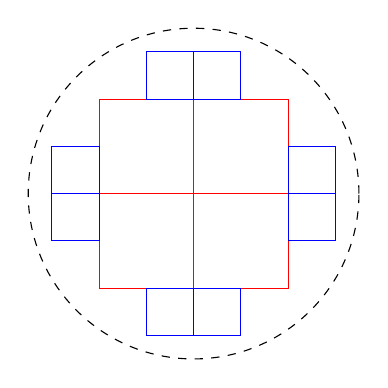
\begin{tikzpicture}[scale=0.6]
            \draw[-, black, dashed] (0,0) circle (3.5);
            \foreach \i in {-2,0} {
                \foreach \j in {-2,0} {
                    \draw[-, red] (\i,\j) rectangle (\i+2, \j+2);
                }        
            }
            \foreach \i in {-1,0} {
                \foreach \j in {-3,2} {
                    \draw[-, blue] (\i,\j) rectangle (\i+1, \j+1);
                    \draw[-, blue] (\j,\i) rectangle (\j+1, \i+1);
                }
            }
        \end{tikzpicture}
        $\mathcal{H}_1 \cup \mathcal{H}_2$
    \end{center}
\end{minipage}
\\[6ex]
Probaremos que \hspace{1mm}
$O = \displaystyle \bigcup_{n \in \N} \hspace{1mm} \bigcup_{C \in \mathcal{H}_n} \hspace{-1mm} C$
\hspace{1mm} por doble contenido.

\begin{tcolorbox}[Subset-contingency]
    $\supseteq$ \hspace{4mm} Por definición de $\mathcal{H}_n$, \hspace{2mm}
    $\forall n \in \N$ se tiene $C \in \mathcal{H}_n \Rightarrow C \subsetneq \overline{C} \subsetneq  O$
\end{tcolorbox}
\begin{tcolorbox}[Subset-contingency]
    $\subseteq $ \hspace{4mm}
    Sea $x_0 \in O \subseteq \R^N$ cualquiera, podemos expresarlo como $x_0 = (x_1, \ldots, x_N)$.
\end{tcolorbox}
Al ser $O$ abierto en $(\R^N, \tau_{\R^N}(d))$, existe $n_0 \in \N$ que verifica:
$$x_0 \in \prod_{i=1}^N \left(x_i - \frac{1}{2^{n_0}},\hspace{1mm}  x_i + \frac{1}{2^{n_0}}\right) \subset \prod_{i=1}^N \left[x_i - \frac{1}{2^{n_0}}, \hspace{1mm} x_i + \frac{1}{2^{n_0}}\right] \subset O$$
Además, para cada coordenada $1 \leq i \leq N$ tenemos que $\exists ! j_i \in \Z : x_i \in \left[\frac{j_i -1}{2^{n_0}}, \frac{j_i}{2^{n_0}} \right)$.
Así, para cada $i \in {1, \ldots, N}$ se tiene que:
\begin{align*}
    \left. \begin{array}{l}
        \frac{j_i - 1}{2^{n_0}} \leq x_i \Rightarrow \frac{j_i}{2^{n_0}} \leq x_i + \frac{1}{2^{n_0}} \\
        x_i < \frac{j_i}{2^{n_0}} \Rightarrow x_i - \frac{1}{2^{n_0}} < \frac{j_i - 1}{2^{n_0}}
    \end{array} \right\} \textstyle
    \Rightarrow \left[\frac{j_i -1}{2^{n_0}}, \frac{j_i}{2^{n_0}} \right) \subset \left(x_i - \frac{1}{2^{n_0}}, x_i + \frac{1}{2^{n_0}} \right)
\end{align*}
De este modo, $D_0 := \displaystyle \prod_{i=1}^{N}\left[\frac{j_i-1}{2^{n_0}}, \frac{j_i}{2^{n_0}} \right) \subsetneq \prod_{i=1}^{N}\left[x_i - \frac{1}{2^{n_0}}, x_i + \frac{1}{2^{n_0}} \right] \subsetneq O$.

\vspace{3mm} \noindent
Y por tanto, $x_0 \in D_0 \subsetneq \overline{D_0} \subsetneq O$. A su vez, como $D_0 \in \mathcal{G}_{n_0}$, hemos demostrado también
que el siguiente conjunto es no vacío: \\[-2.5ex]
$$\mathcal{A}_{x_0} := \Big\{n \in \N : \exists \hspace{1mm} C \in \mathcal{G}_n \text{ tal que } x_0 \in C\Big\} $$

\vspace{4mm}
Al ser $A_{x_0}$ un subconjunto no vacío de $\N$, podemos afirmar que tiene mínimo, al que denotaremos $m_0$. Así, ha de existir $C_0 \in \mathcal{G}_{m_0}$ tal que $x_0 \in C_0$, veamos
que $C_0 \in \mathcal{H}_{m_0}$. Por definición de $\mathcal{H}_{m_0}$, $C_0 \notin \mathcal{H}_{m_0} \Rightarrow C_0 \in \mathcal{G}_n$ para cierto $n < m_0$. Esto contradice
que $m_0$ sea el mínimo de $\mathcal{A}_{x_0}$. Hemos demostrado que $C_0 \in \mathcal{H}_{m_0}$.

\newpage
\chapter{Series dobles}
El álgebra contempla únicamente la suma como operación binaria. Por la propiedad asociativa, es posible expresar cualquier suma finita como sumas binarias sucesivas.
Para No obstante, el álgebra por sí misma no nos basta para sumar series.

\vspace{4mm}
\result{Definición de sucesión doble}
\hspace{3mm} Llamamos ``sucesión doble'' a cualquier aplicación
\begin{flalign*}
    \hspace{2mm} \gamma : \N \times \N &\longrightarrow \overline{\R} = \R \cup \{+\infty -\infty\} &&\\
    \hspace{2mm} n, m &\longmapsto \gamma(n,m) = a_{nm} &&
\end{flalign*} \\[-5ex]
Diremos que $a_{nm}$ es el término general de la sucesión.

\vspace{4mm}
\result{Definición de serie doble}
\hspace{3mm} Dada una sucesión doble de término general $a_{nm}$, llamamos ``serie doble de término general $a_{nm}$''
a la expresión $\displaystyle \sum_{n,m} a_{nm}$ (que equivale a $\displaystyle \sum_{\substack{n = 1\\m=1}}a_{nm}$ \hspace{2mm}).

\vspace{4mm}
Diremos que $\sum_{n,m}a_{nm}$ es convergente si sus sumas parciales convergen a un número real. Es decir, si:
$\exists s \in \R $ que verifica: \\[-4ex]
$$ \forall\hspace{1mm}\varepsilon > 0 \hspace{2mm} \exists \hspace{1mm} n_0 \in \N \text{ tal que }\hspace{2mm}  n,m \geq n_0 \Rightarrow
\left|s - \sum_{\substack{1\leq i \leq n\\1\leq j \leq n}}a_{ij}\right| < \varepsilon$$
En este caso, diremos que este $s$ es el ``valor de la suma de la serie''.

\vspace{4mm}
Diremos que $\sum_{n,m} a_{nm}$ es divergente a $+\infty (-\infty)$ si $\forall \hspace{1mm} \in \R$
$\exists \hspace{1mm} n_0  \in \N$ tal que dados $n, m \geq n_0$ se cumple: \\[-5ex]
\begin{align*}
    \sum_{\substack{1\leq i \leq n\\1 \leq j \leq m}}a_{ij} > K &&
    \left(\sum_{\substack{1\leq i \leq n\\1 \leq j \leq m}}a_{ij} < K\right)
\end{align*}
En este caso, diremos que el valor de la suma de la sucesión es $+\infty (-\infty)$.

Es importante distinguir la igualdad de series como sucesiones y como valores. Veamos un ejemplo
con series simples: \\[-5ex]
\begin{align*}
    \sum_{n=1}^\infty a_n = 1 +0+0+0+\ldots &&
    \sum_{n=1}^\infty b_n = \frac{1}{2} + \frac{1}{4} + \frac{1}{8} + \frac{1}{16} + \ldots
\end{align*} \\[-4ex]
Es claro que las series no tienen el mismo término general (no son iguales como series), pero sí tienen el mismo valor de suma (que es 1).

\vspace{6mm}
\result{Teorema de series dobles no negativas}
\hspace{3mm} Dada una sucesión doble $\gamma : \N \times \N \longrightarrow [0, +\infty]$ de término general $a_{nm}$,
dada una biyección cualquiera $g : \N \longrightarrow \N \times \N$, se cumple:
\begin{align*}
    \sum_{n,m} a_{nm} = \sum_{n = 1}^{\infty}a_{g(n)} = \sum_{n=1}^{\infty}\sum_{m=1}^{\infty}a_{nm} = \sum_{m=1}^{\infty}\sum_{n=1}^{\infty}a_{nm} \in[0, +\infty]
\end{align*}
\dem Probaremos primero la igualdad respecto de la reordenación y después respecto de las series anidadas.

\vspace{2mm}
Si existe algún término $a_{n_0m_0} = +\infty$, entonces la igualdad se cumple trivialmente al estar las sumas bien definidas ($\gamma(\N \times \N) \subseteq[0, +\infty])$.
Supongamos entonces que todos los términos son finitos, veamos qué casos pueden darse:

\vspace{5mm}
$\bullet$ Primer caso: Supongamos que $\displaystyle{\sum_{n=1}^{\infty}a_{g(n)}} = s \in \R$.

\noindent
Por definición, $\forall \varepsilon > 0 \hspace{1mm} \exists \hspace{1mm} n_0 \in \N : \hspace{2mm} s - \displaystyle{\sum_{k=1}^{n}a_{g(k)}} < \varepsilon \hspace{2mm} \forall n \geq n_0$.
Sea $\varepsilon > 0$ cualquiera pero fijo, fijamos también el $n_0$ asociado.
Como $g$ es biyectiva, $\exists \hspace{1mm} m_0 \in \N$ tal que $g(\{1,\ldots,n_0\}) \subseteq \{1,\ldots, m_0\} \times \{1,\ldots,m_0\}$.
Al tratarse de series de términos no negativos, dados $n,m \in \N$ con $n\geq n_0, m\geq n_0$, se cumple:
$$\sum_{k=1}^{n_0}a_{g(k)} \leq \sum_{\substack{1\leq i \leq n\\1\leq j \leq m}}a_{ij}
\Rightarrow 0 \overset{(*)}{\leq} s -  \sum_{\substack{1\leq i \leq n\\1\leq j \leq m}}a_{ij} \leq s - \sum_{k=1}^{n_0}a_{g(k)} < \varepsilon$$
(*) La desigualdad se deduce de que la suma parcial de la serie doble es una reordenación de la suma parcial de la serie simple, siendo esta última absolutamente convergente.
Como podemos hacer $\varepsilon$ arbitrariamente pequeño, concluimos que las dos series tienen el mismo límite.

\vspace{4mm}
$\bullet$ Segundo caso: $\sum_{n=1}\infty a_{g(n)} = +\infty$.

\vspace{2mm}
Sea $K \in \R$, por definición, $\exists \hspace{1mm} n_0 \in \N \text{ tal que } \sum_{k=1}^{n} a_{g(k)} > K \hspace{2mm} \forall \hspace{1mm} n \geq n_0$.
AL ser $g$ biyectiva, $\exists \hspace{1mm} m_0 \in \N \text{ tal que } g({1,\ldots,n_0}) \subseteq \{1,\ldots, m_0\} \times \{1,\ldots,m_0\}$. Así, dados $n \geq m_0, m\geq m_0$ se tiene:
\\[-3ex] $$K < \sum_{k=1}^{n_0} a_{g(k)} \leq \sum_{\substack{1\leq i \leq n\\1\leq j \leq m}} a_{ij}$$
Es claro que la serie doble diverge a $+\infty$.

\vspace{4mm}
Queda probar la igualdad entre la serie doble y las series anidadas cuando todos los términos son finitos. Veamos qué ocurre según el carácter de la serie doble.

\vspace{4mm}
$\bullet$ Primer caso: $\sum_{n,m}a_{nm} = s \in [0,+\infty)$.

\vspace{2mm}
Sea $\varepsilon > 0$. Por definición de convergencia, sabemos que
$\exists \hspace{1mm} n_0 \in \N \text{ tal que dados } n\geq n_0, m\geq n_0$ se tiene:
$$\left|\hspace{1mm} s - \sum_{\substack{1\leq i \leq n\\1\leq j \leq m}} a_{ij} \hspace{1mm} \right| < \varepsilon$$
\\[1mm]
Nótese que debido a las propiedades algebraicas de la suma, en el caso finito se da la igualdad; es decir:
\\[-3.5ex]
$$\sum_{\substack{1\leq i \leq n\\1\leq j \leq m}} a_{ij} = \sum_{i=1}^n\sum_{j=1}^m a_{ij} = \sum_{j=1}^m\sum_{i=1}^n a_{ij}$$
De este modo, sustituyendo en la definición de convergencia, dados $n \geq n_0, m\geq n_0$ obtenemos:
\begin{flalign*}
    \left|\hspace{1mm}s- \sum_{j=1}^m\sum_{i=1}^n a_{ij} \hspace{1mm}\right| < \varepsilon
    \Rightarrow \varepsilon \geq \lim_n \left|\hspace{1mm} s - \sum_{j=1}^m\sum_{i=1}^n a_{ij} \hspace{1mm}\right|
    = \left|\hspace{1mm} s - \sum_{j=1}^m \lim_n \left( \sum_{i=1}^n a_{ij} \right)\hspace{1mm}\right|
\end{flalign*}
La igualdad se debe a aplicar las propiedades del límite con funciones continuas. Como la serie doble converge por hipótesis,
también han de hacerlo las series de filas y columnas. Es por ello que podemos afirmar que el último límite existe.

\vspace{2mm}
La igualdad anterior se cumple para cualquier $\varepsilon > 0$ y para cualquier $m \geq n_0$. Haciendo $\varepsilon$
arbitrariamente pequeño y tomando límites en $m$ llegamos al resultado. El razonamiento para la otra serie anidada es análogo; así, concluimos:
\begin{flalign*}
    \sum_{m=1}^\infty\sum_{n=1}^\infty a_{nm} = \sum_{n=1}^{\infty}\sum_{m=1}^{\infty}a_{nm} = \sum_{n,m}a_{nm}
\end{flalign*}

\vspace{4mm}
$\bullet$ Segundo caso: $\sum_{n,m}a_{nm} = +\infty$. Si hubiese algún $n\in \N$ verificando $\sum_{m=1}^\infty a_{nm} = +\infty$ 
o si existiese algún $m \in \N$ tal que $\sum_{n=1}^{\infty}a_{nm} = +\infty$, las series anidadas divergerían trivialmente.
Supongamos que no es el caso para ver que también se cumple el resultado.

\vspace{2mm}
Sea $K \in \R$ cualquiera, por definición de divergencia se cumple:
\begin{flalign*}
    \exists \hspace{1mm} n_0 \in \N \text{ tal que } \forall \hspace{1mm} n \geq n_0, \forall m \geq n_0 \text{ se cumple } \sum_{j=1}^{m}\sum_{i=1}^n a_{ij} > K
\end{flalign*}
Nótese que hemos utilizado la igualdad entre la serie doble y las series anidadas para el caso finito. Además, dados $n \geq n_0, m \geq n_0$, se cumple:
\begin{flalign*}
    \sum_{j=1}^{m}\sum_{i=1}^{n} a_{ij} > K
    \Rightarrow K \leq \lim_n \sum_{j=1}^{m}\sum_{i=1}^{n} a_{ij}
    = \sum_{j=1}^{m} \left( \sum_{i=1}^{\infty} a_{ij}\right)
\end{flalign*}
Las series de suma de filas y columnas existen por hipótesis, luego la igualdad se cumple para todo $m \geq n_0$. Tomando límites en $m$ podemos observar que
$\sum_{m=1}^\infty \sum_{n=1}^\infty a_{nm} \geq K$. Como el $K$ escogido fue arbitrario, se cumple para cualquier $K$ real.
Así, las series anidadas divergen a $+\infty$ (análogo para la otra serie anidada).

\newpage
\unit{Teoría de la medida}

\vspace{2mm}
\chapter{Espacios de medida}
\result{Definición de \texorpdfstring{$\sigma$}{s}-álgebra}
\hspace{3mm} Sea $X$ un conjunto cualquiera, diremos que $\Sigma \subseteq \mathcal{P}(X)$ es una $\sigma$-álgebra si cumple las siguientes propiedades:
\begin{enumerate}[label=S.\arabic*)]
    \item $\varnothing \in \Sigma$
    \item $\left\{E_i : i\in \N\right\} \subseteq \Sigma \Rightarrow \displaystyle{\bigcup_{i \in \N}{E_i}} \in \Sigma$
    \item $E \in \Sigma \Rightarrow E^c := X \backslash E \in \Sigma$
\end{enumerate}
Nótese que no es necesario exigir que $X$ tenga ningún tipo de estructura (ni topológica, ni algebraica...).

\vspace{4mm}
\result{Propiedades de las \texorpdfstring{$\sigma$}{s}-álgebras}
\hspace{3mm} Sea $X$ un conjunto, sea $\Sigma$ una $\sigma$-álgebra de $X$.
Sea $\{E_i : i \in \N\} \subseteq \Sigma$, y $E,F \in \Sigma$. Entonces, se cumple:
\begin{enumerate}[label=\roman*)]
    \item $\displaystyle{\bigcap_{i\in\N}{E_i}} \in \Sigma$
    \item $E\cup F \in \Sigma$
    \item $E \cap F \in \Sigma$
    \item $E \backslash F \in \Sigma$
\end{enumerate}

\vspace{2mm} \dem

\vspace{2mm}
$\romannumeral 1)$ Por la propiedad $(S.3)$ y la involución del complementario, un conjunto pertenece a una $\sigma$-álgebra si y solo si su complementario pertenece a ella.
Por tanto, basta ver que: \hspace{2mm}
$X \setminus \left(\bigcap_{i\in\N}{E_i}\right)
= \displaystyle{\bigcup_{i\in\N}{\left(X \setminus E_i\right)}} \in \Sigma$.

Por la propiedad $(S.3)$, para cada $i \in \N$ tenemos que $X\setminus E_i \in \Sigma$, pues $E_i \in \Sigma$ por hipótesis.
Finalmente, aplicando $(S.1)$ tenemos que su unión numerable se encuentra en $\Sigma$.

\vspace{4mm}
$\romannumeral 2)$ Reescribiremos $E\cup F$ para hacer uso del resultado que acabamos de probar.
Por $(S.1)$ sabemos que $\varnothing \in \Sigma$ luego podemos considerar la colección numerable de conjuntos de $\Sigma$,
$\{A_i : i \in \N\}$ donde $A_1 = E, \hspace{2mm} A_2 = F$, y $ A_n = \varnothing  \hspace{2mm} \forall \hspace{1mm} n > 2$.

\vspace{2mm} \noindent
De este modo, $E \cup F = E \cup F \cup \varnothing  \cup \varnothing \cup \ldots = \displaystyle{\bigcup_{i \in \N}{A_i}} \in \Sigma$.

\vspace{4mm}
$\romannumeral 3)$ Como consecuencia de $(S.1)$ y de $(S.3)$, sabemos que $X \in \Sigma$.
Así, basta considerar $B_1 = E,$ $B_2 = F$, $B_n = X \hspace{2mm} \forall \hspace{1mm} n > 2$.

\vspace{2mm} \noindent
Aplicando el apartado $(\romannumeral 1)$, $E \cap F = E \cap F \cap X \cap X \cap \ldots
= \displaystyle{\bigcap_{i \in \N}{B_i}} \in \Sigma$.

\vspace{4mm}
$\romannumeral 4)$ Por definición de complementario, $E\setminus F = E \cap (X \setminus F)$.
Por hipótesis, $E,F\in \Sigma$. Aplicando $(S.3)$, $(X\setminus F)\in \Sigma$.
Finalmente, aplicando el apartado $(\romannumeral 3)$, $E \cap (X \setminus F) \in \Sigma$.

\vspace{6mm}
\result{Definición de espacio de medida}
\hspace{3mm} Sea $X$ un conjunto cualquiera y $\Sigma$ una $\sigma$-álgebra de $X$, diremos que
$\mu : \Sigma \longrightarrow [0,+\infty]$ es una medida sobre $\Sigma$ si verifica las siguientes propiedades:
\begin{enumerate}[label=M.\arabic*)]
    \item $\mu(\varnothing) = 0$
    \item Sean $\{E_i : i\in \N\} \subseteq \Sigma$ tales que $i \neq j \Rightarrow E_i \cap E_j = \varnothing $; entonces,
    $$\mu\left(\bigcup_{i\in \N} E_i\right) = \sum_{i\in \N} \mu(E_i)$$
\end{enumerate}

\vspace{2mm}
A la tríada $(X, \Sigma, \mu)$ se la denomina ``espacio de medida'', y a los conjuntos
de $\Sigma$ se los llama ``conjuntos ($\mu$-medibles) de $X$''.

\result{Propiedades de los espacios de medida}
\hspace{3mm} Sea $(X,\Sigma,\mu)$ un espacio de medida, se cumple:
\begin{enumerate}[label=\roman*)]
    \item Sean $E,F\in \Sigma$ con $F \subseteq E$, se cumple $\mu(F) \leq \mu(E)$.
    \newline \noindent
    Si además se tiene que $\mu(F) < +\infty$, entonces $\mu(E \setminus F) = \mu(E) - \mu(F)$.
    
    \item Sean $\{E_i : i \in \N\} \subseteq \Sigma$ tales que $E_i \subseteq E_{i+1} \hspace{2mm}\forall \hspace{1mm} i \in \N$.
    \newline\noindent
    Entonces, $\mu (\smallcup_{i \in \N}{E_i}) = \displaystyle{\lim_n \mu(E_n)}$.
    
    \item Sean $\{E_i : i \in \N\} \subseteq \Sigma$ tales que $E_{i+1} \subseteq E_{i} \hspace{2mm}\forall \hspace{1mm} i \in \N$, y $\mu(E_1) < +\infty$.
    \newline \noindent
    Entonces, $\mu(\smallcap_{i\in\N}E_i) = \mlim{n} \hspace{1mm} \mu(E_n)$.
\end{enumerate}

\vspace{2mm} \dem

\vspace{2mm}
$\romannumeral 1)$ Reescribiendo como unión numerable
de conjuntos disjuntos de $\Sigma$, \\[-5ex]
\begin{flalign*}
    E = (E \setminus F) \cup F \cup \varnothing \cup \varnothing \cup\ldots 
\end{flalign*}
\\[-5ex]
Aplicando $(M.3)$ y evaluando $\mu$ a ambos lados obtenemos:
\\[-5ex]
\begin{flalign*}
    \mu(E) = \mu(E \setminus F) + \mu(F) + \mu(\varnothing) + \mu(\varnothing) + \ldots    
\end{flalign*}
Aplicando $(M.1)$ se deduce que $\mu(E) = \mu(E \setminus F) + \mu(F)$.
Por la no negatividad de $\mu$, se tiene que $\hspace{1mm} \mu(E \setminus F) \geq 0 \Rightarrow \mu(F) \leq \mu(F)$.

\vspace{2mm} \noindent
Si además $\mu(F) < +\infty$, podemos despejar sin que ocurran indeterminaciones; así, $\mu(E \setminus F) = \mu(E) - \mu(F)$.

\vspace{8mm}
$\romannumeral 2)$ Una vez más, reescribimos el conjunto a partir de uniones disjuntas:
$$\bigcup_{i\in \N} E_i = E_1 \cup \Big(E_2 \setminus E_1\Big) \cup \Big(E_3 \setminus (E_2 \cup E_1)\Big)
\cup \Big(E_4 \setminus (E_1 \cup E_2 \cup E_3)\Big) \cup \ldots$$
Como $E_i \subseteq E_{i+1}$ por hipótesis, podemos simplificar esta expresión: \\[-3ex]
$$\bigcup_{i\in \N}E_i = E_1 \cup (E_2 \setminus E_1) \cup (E_3 \setminus E_2)
\cup (E_4 \setminus E_3)\cup \ldots = E_1 \cup \left(\bigcup_{i \in \N}(E_{i+1}\setminus E_i)\right)$$
Así, $\hspace{2mm} \displaystyle \mu\left(\bigcup_{i\in\N}E_i\right)= \mu(E_1) + \sum_{i=2}^{\infty}\mu(E_{i}\setminus E_{i-1}) = (*)$.

\noindent
Distinguimos dos casos en función de la medida de los $E_i$:

\vspace{2mm}
$\romannumeral 2.a)$ Existe cierto $j \in \N$ tal que $\mu(E_j) = +\infty$.
Como $E_j \subseteq E_n \hspace{2mm} \forall \hspace{1mm} n \geq j$, aplicando \hyperref[result:1.4.4]{las propiedad $(i)$ de la medida},
se tiene que $\mu(E_n) = +\infty \hspace{2mm} \forall \hspace{1mm} n \geq j$,
luego ha de cumplirse $\mlim{n} \hspace{1mm}\mu(E_n) = +\infty$.
Por otro lado, como $E_j \subseteq \smallcup_{i\in \N} E_i$, se tiene que
$+\infty = \mu(E_j) \leq \mu(\smallcup_{i\in\N}E_i)$,
luego, $\mlim{n} \hspace{1mm} \mu(E_n) = \mu(\smallcup_{i\in\N}E_i) = +\infty$.

\vspace{4mm}
$\romannumeral 2.b)$ En caso contrario al anterior, $\mu(E_i) < +\infty \hspace{2mm} \forall \hspace{1mm} i \in \N$. Desarrollando en $(*)$,
\begin{flalign*}
    \mu\Big(\smallcup_{i\in\N} &E_i\Big) = \mu(E_1) + \sum_{i=2}^{\infty}\mu(E_{i}\setminus E_{i-1})
    = \mu(1) + \lim_n \sum_{i=2}^{n}\mu(E_i \setminus E_{i-1}) = \\
    &= \lim_n \Big(\mu(E_1) + \mu(E_2 \setminus E_1) + \mu(E_3 \setminus E_2) + \ldots + \mu(E_{n} \setminus E_{n-1}) \Big) = \\
    &= \lim_n \Big(\mu(E_1) + \big(\mu(E_2) - \mu(E_1)\big) + \ldots + \big(\mu(E_n) - \mu(E_{n-1})\big)\Big) = \\
    &= \lim_n \mu(E_n)
\end{flalign*}
Hemos podido simplificar porque todas las medidas son finitas; de lo contrario, podrían producirse indeterminaciones.

\vspace{8mm}
$\romannumeral 3)$ Por hipótesis, $E_{i+1} \subseteq E_i \hspace{2mm} \forall \hspace{1mm} i \in \N$, y $\mu(E_1) < +\infty$.
De este modo, como todos los $E_i$ son subconjuntos de $E_1$ han de tener medida finita también (\hyperref[result:1.1.4]{propiedad $(i)$ de la medida}).
Expresamos la intersección según el complementario respecto de $E_1$ como sigue:
$\hspace{2mm} E_1 \setminus \big(\smallcap_{i\in\N}E_i\big) = \smallcup_{i\in\N}\big(E_1 \setminus E_i\big)$.

\vspace{4mm} \noindent
Por hipótesis, $E_{i+1} \subseteq E_i \Rightarrow (E_1 \setminus E_i) \subseteq (E_1\setminus E_{i+1})$.
Como consecuencia, aplicando los apartados anteriores de este resultado,
\begin{flalign*}
    \mu(E_1) - \mu\Big(\smallcap_{i\in\N}E_i\Big)
    &=\mu\Big(E_1 \setminus\big(\smallcap_{i\in\N}E_i\big)\Big)
    = \mu\Big(\smallcup_{i\in\N}(E_1 \setminus E_i)\Big) =\\[1ex]
    &= \lim_n \mu(E_1 \setminus E_n)
    = \mu(E_1) - \lim_n \mu(E_n)
\end{flalign*}
Como todas las medidas son finitas, podemos despejar sin indeterminaciones: 
$$\mu\Big(\smallcap_{i\in\N}E_i\Big) = \lim_n \mu(E_n)$$
\end{document}